% !TEX root = tnnls_relation_gait.tex

\ifx\allfiles\undefined
    % !TEX root = tnnls_relation_gait.tex

%% bare_jrnl.tex
%% V1.4b
%% 2015/08/26
%% by Michael Shell
%% see http://www.michaelshell.org/
%% for current contact information.
%%
%% This is a skeleton file demonstrating the use of IEEEtran.cls
%% (requires IEEEtran.cls version 1.8b or later) with an IEEE
%% journal paper.
%%
%% Support sites:
%% http://www.michaelshell.org/tex/ieeetran/
%% http://www.ctan.org/pkg/ieeetran
%% and
%% http://www.ieee.org/

%%*************************************************************************
%% Legal Notice:
%% This code is offered as-is without any warranty either expressed or
%% implied; without even the implied warranty of MERCHANTABILITY or
%% FITNESS FOR A PARTICULAR PURPOSE!
%% User assumes all risk.
%% In no event shall the IEEE or any contributor to this code be liable for
%% any damages or losses, including, but not limited to, incidental,
%% consequential, or any other damages, resulting from the use or misuse
%% of any information contained here.
%%
%% All comments are the opinions of their respective authors and are not
%% necessarily endorsed by the IEEE.
%%
%% This work is distributed under the LaTeX Project Public License (LPPL)
%% ( http://www.latex-project.org/ ) version 1.3, and may be freely used,
%% distributed and modified. A copy of the LPPL, version 1.3, is included
%% in the base LaTeX documentation of all distributions of LaTeX released
%% 2003/12/01 or later.
%% Retain all contribution notices and credits.
%% ** Modified files should be clearly indicated as such, including  **
%% ** renaming them and changing author support contact information. **
%%*************************************************************************


% *** Authors should verify (and, if needed, correct) their LaTeX system  ***
% *** with the testflow diagnostic prior to trusting their LaTeX platform ***
% *** with production work. The IEEE's font choices and paper sizes can   ***
% *** trigger bugs that do not appear when using other class files.       ***                          ***
% The testflow support page is at:
% http://www.michaelshell.org/tex/testflow/

\documentclass[journal]{IEEEtran}
%
% If IEEEtran.cls has not been installed into the LaTeX system files,
% manually specify the path to it like:
% \documentclass[journal]{../sty/IEEEtran}

% Some very useful LaTeX packages include:
% (uncomment the ones you want to load)

% *** MISC UTILITY PACKAGES ***
%
%\usepackage{ifpdf}
% Heiko Oberdiek's ifpdf.sty is very useful if you need conditional
% compilation based on whether the output is pdf or dvi.
% usage:
% \ifpdf
%   % pdf code
% \else
%   % dvi code
% \fi
% The latest version of ifpdf.sty can be obtained from:
% http://www.ctan.org/pkg/ifpdf
% Also, note that IEEEtran.cls V1.7 and later provides a builtin
% \ifCLASSINFOpdf conditional that works the same way.
% When switching from latex to pdflatex and vice-versa, the compiler may
% have to be run twice to clear warning/error messages.

% *** CITATION PACKAGES ***

\usepackage{tabularx}
\usepackage{longtable}
\usepackage{threeparttable}
\usepackage{cite}

% cite.sty was written by Donald Arseneau
% V1.6 and later of IEEEtran pre-defines the format of the cite.sty package
% \cite{} output to follow that of the IEEE. Loading the cite package will
% result in citation numbers being automatically sorted and properly
% "compressed/ranged". e.g., [1], [9], [2], [7], [5], [6] without using
% cite.sty will become [1], [2], [5]--[7], [9] using cite.sty. cite.sty's
% \cite will automatically add leading space, if needed. Use cite.sty's
% noadjust option (cite.sty V3.8 and later) if you want to turn this off
% such as if a citation ever needs to be enclosed in parenthesis.
% cite.sty is already installed on most LaTeX systems. Be sure and use
% version 5.0 (2009-03-20) and later if using hyperref.sty.
% The latest version can be obtained at:
% http://www.ctan.org/pkg/cite
% The documentation is contained in the cite.sty file itself.

% *** GRAPHICS RELATED PACKAGES ***
%
\usepackage[pdftex]{graphicx}
\usepackage{rotating}
\ifCLASSINFOpdf
  % \usepackage[pdftex]{graphicx}
  % declare the path(s) where your graphic files are
  % \graphicspath{{../pdf/}{../jpeg/}}
  % and their extensions so you won't have to specify these with
  % every instance of \includegraphics
  % \DeclareGraphicsExtensions{.pdf,.jpeg,.png}
\else
  % or other class option (dvipsone, dvipdf, if not using dvips). graphicx
  % will default to the driver specified in the system graphics.cfg if no
  % driver is specified.
  % \usepackage[dvips]{graphicx}
  % declare the path(s) where your graphic files are
  % \graphicspath{{../eps/}}
  % and their extensions so you won't have to specify these with
  % every instance of \includegraphics
  % \DeclareGraphicsExtensions{.eps}
\fi
% graphicx was written by David Carlisle and Sebastian Rahtz. It is
% required if you want graphics, photos, etc. graphicx.sty is already
% installed on most LaTeX systems. The latest version and documentation
% can be obtained at:
% http://www.ctan.org/pkg/graphicx
% Another good source of documentation is "Using Imported Graphics in
% LaTeX2e" by Keith Reckdahl which can be found at:
% http://www.ctan.org/pkg/epslatex
%
% latex, and pdflatex in dvi mode, support graphics in encapsulated
% postscript (.eps) format. pdflatex in pdf mode supports graphics
% in .pdf, .jpeg, .png and .mps (metapost) formats. Users should ensure
% that all non-photo figures use a vector format (.eps, .pdf, .mps) and
% not a bitmapped formats (.jpeg, .png). The IEEE frowns on bitmapped formats
% which can result in "jaggedy"/blurry rendering of lines and letters as
% well as large increases in file sizes.
%
% You can find documentation about the pdfTeX application at:
% http://www.tug.org/applications/pdftex

% *** MATH PACKAGES ***
%
\usepackage{amsmath}
% A popular package from the American Mathematical Society that provides
% many useful and powerful commands for dealing with mathematics.
%
% Note that the amsmath package sets \interdisplaylinepenalty to 10000
% thus preventing page breaks from occurring within multiline equations. Use:
%\interdisplaylinepenalty=2500
% after loading amsmath to restore such page breaks as IEEEtran.cls normally
% does. amsmath.sty is already installed on most LaTeX systems. The latest
% version and documentation can be obtained at:
% http://www.ctan.org/pkg/amsmath

% *** SPECIALIZED LIST PACKAGES ***
%
\usepackage{algorithmic}
% algorithmic.sty was written by Peter Williams and Rogerio Brito.
% This package provides an algorithmic environment fo describing algorithms.
% You can use the algorithmic environment in-text or within a figure
% environment to provide for a floating algorithm. Do NOT use the algorithm
% floating environment provided by algorithm.sty (by the same authors) or
% algorithm2e.sty (by Christophe Fiorio) as the IEEE does not use dedicated
% algorithm float types and packages that provide these will not provide
% correct IEEE style captions. The latest version and documentation of
% algorithmic.sty can be obtained at:
% http://www.ctan.org/pkg/algorithms
% Also of interest may be the (relatively newer and more customizable)
% algorithmicx.sty package by Szasz Janos:
% http://www.ctan.org/pkg/algorithmicx

% *** ALIGNMENT PACKAGES ***
%
\usepackage{array}
% Frank Mittelbach's and David Carlisle's array.sty patches and improves
% the standard LaTeX2e array and tabular environments to provide better
% appearance and additional user controls. As the default LaTeX2e table
% generation code is lacking to the point of almost being broken with
% respect to the quality of the end results, all users are strongly
% advised to use an enhanced (at the very least that provided by array.sty)
% set of table tools. array.sty is already installed on most systems. The
% latest version and documentation can be obtained at:
% http://www.ctan.org/pkg/array

% IEEEtran contains the IEEEeqnarray family of commands that can be used to
% generate multiline equations as well as matrices, tables, etc., of high
% quality.

% *** SUBFIGURE PACKAGES ***
\usepackage[caption=false,font=footnotesize]{subfig}
%\ifCLASSOPTIONcompsoc
%  \usepackage[caption=false,font=normalsize,labelfont=sf,textfont=sf]{subfig}
%\else
%  \usepackage[caption=false,font=footnotesize]{subfig}
%\fi
% subfig.sty, written by Steven Douglas Cochran, is the modern replacement
% for subfigure.sty, the latter of which is no longer maintained and is
% incompatible with some LaTeX packages including fixltx2e. However,
% subfig.sty requires and automatically loads Axel Sommerfeldt's caption.sty
% which will override IEEEtran.cls' handling of captions and this will result
% in non-IEEE style figure/table captions. To prevent this problem, be sure
% and invoke subfig.sty's "caption=false" package option (available since
% subfig.sty version 1.3, 2005/06/28) as this is will preserve IEEEtran.cls
% handling of captions.
% Note that the Computer Society format requires a larger sans serif font
% than the serif footnote size font used in traditional IEEE formatting
% and thus the need to invoke different subfig.sty package options depending
% on whether compsoc mode has been enabled.
%
% The latest version and documentation of subfig.sty can be obtained at:
% http://www.ctan.org/pkg/subfig

% *** FLOAT PACKAGES ***
%
%\usepackage{fixltx2e}
% fixltx2e, the successor to the earlier fix2col.sty, was written by
% Frank Mittelbach and David Carlisle. This package corrects a few problems
% in the LaTeX2e kernel, the most notable of which is that in current
% LaTeX2e releases, the ordering of single and double column floats is not
% guaranteed to be preserved. Thus, an unpatched LaTeX2e can allow a
% single column figure to be placed prior to an earlier double column
% figure.
% Be aware that LaTeX2e kernels dated 2015 and later have fixltx2e.sty's
% corrections already built into the system in which case a warning will
% be issued if an attempt is made to load fixltx2e.sty as it is no longer
% needed.
% The latest version and documentation can be found at:
% http://www.ctan.org/pkg/fixltx2e

%\usepackage{stfloats}
% stfloats.sty was written by Sigitas Tolusis. This package gives LaTeX2e
% the ability to do double column floats at the bottom of the page as well
% as the top. (e.g., "\begin{figure*}[!b]" is not normally possible in
% LaTeX2e). It also provides a command:
%\fnbelowfloat
% to enable the placement of footnotes below bottom floats (the standard
% LaTeX2e kernel puts them above bottom floats). This is an invasive package
% which rewrites many portions of the LaTeX2e float routines. It may not work
% with other packages that modify the LaTeX2e float routines. The latest
% version and documentation can be obtained at:
% http://www.ctan.org/pkg/stfloats
% Do not use the stfloats baselinefloat ability as the IEEE does not allow
% \baselineskip to stretch. Authors submitting work to the IEEE should note
% that the IEEE rarely uses double column equations and that authors should try
% to avoid such use. Do not be tempted to use the cuted.sty or midfloat.sty
% packages (also by Sigitas Tolusis) as the IEEE does not format its papers in
% such ways.
% Do not attempt to use stfloats with fixltx2e as they are incompatible.
% Instead, use Morten Hogholm'a dblfloatfix which combines the features
% of both fixltx2e and stfloats:
%
% \usepackage{dblfloatfix}
% The latest version can be found at:
% http://www.ctan.org/pkg/dblfloatfix

%\ifCLASSOPTIONcaptionsoff
%  \usepackage[nomarkers]{endfloat}
% \let\MYoriglatexcaption\caption
% \renewcommand{\caption}[2][\relax]{\MYoriglatexcaption[#2]{#2}}
%\fi
% endfloat.sty was written by James Darrell McCauley, Jeff Goldberg and
% Axel Sommerfeldt. This package may be useful when used in conjunction with
% IEEEtran.cls'  captionsoff option. Some IEEE journals/societies require that
% submissions have lists of figures/tables at the end of the paper and that
% figures/tables without any captions are placed on a page by themselves at
% the end of the document. If needed, the draftcls IEEEtran class option or
% \CLASSINPUTbaselinestretch interface can be used to increase the line
% spacing as well. Be sure and use the nomarkers option of endfloat to
% prevent endfloat from "marking" where the figures would have been placed
% in the text. The two hack lines of code above are a slight modification of
% that suggested by in the endfloat docs (section 8.4.1) to ensure that
% the full captions always appear in the list of figures/tables - even if
% the user used the short optional argument of \caption[]{}.
% IEEE papers do not typically make use of \caption[]'s optional argument,
% so this should not be an issue. A similar trick can be used to disable
% captions of packages such as subfig.sty that lack options to turn off
% the subcaptions:
% For subfig.sty:
% \let\MYorigsubfloat\subfloat
% \renewcommand{\subfloat}[2][\relax]{\MYorigsubfloat[]{#2}}
% However, the above trick will not work if both optional arguments of
% the \subfloat command are used. Furthermore, there needs to be a
% description of each subfigure *somewhere* and endfloat does not add
% subfigure captions to its list of figures. Thus, the best approach is to
% avoid the use of subfigure captions (many IEEE journals avoid them anyway)
% and instead reference/explain all the subfigures within the main caption.
% The latest version of endfloat.sty and its documentation can obtained at:
% http://www.ctan.org/pkg/endfloat
%
% The IEEEtran \ifCLASSOPTIONcaptionsoff conditional can also be used
% later in the document, say, to conditionally put the References on a
% page by themselves.

% *** PDF, URL AND HYPERLINK PACKAGES ***
%
\usepackage{url}
% url.sty was written by Donald Arseneau. It provides better support for
% handling and breaking URLs. url.sty is already installed on most LaTeX
% systems. The latest version and documentation can be obtained at:
% http://www.ctan.org/pkg/url
% Basically, \url{my_url_here}.

% *** Do not adjust lengths that control margins, column widths, etc. ***
% *** Do not use packages that alter fonts (such as pslatex).         ***
% There should be no need to do such things with IEEEtran.cls V1.6 and later.
% (Unless specifically asked to do so by the journal or conference you plan
% to submit to, of course. )

% correct bad hyphenation here
% \hyphenation{op-tical net-works semi-conduc-tor}
\usepackage{enumerate}
\usepackage{multirow}
\usepackage{color}
\usepackage{threeparttable}
\usepackage{booktabs}
\newcommand{\minus}{\scalebox{0.75}[1.0]{$-$}}
\newcommand{\bftab}[1]{{\fontseries{b}\selectfont#1}}
\newcommand{\tabincell}[2]{\begin{tabular}{@{}#1@{}}#2\end{tabular}}
\newcommand{\etal}{\textit{et al}.}
\newcommand{\ie}{\textit{i.e.}}
\newcommand{\eg}{\textit{e.g.}}
\newcommand{\wrt}{\textit{w.r.t.}}
\newcommand{\vs}{\textit{vs.}}


\begin{document}
%
% paper title
% Titles are generally capitalized except for words such as a, an, and, as,
% at, but, by, for, in, nor, of, on, or, the, to and up, which are usually
% not capitalized unless they are the first or last word of the title.
% Linebreaks \\ can be used within to get better formatting as desired.
% Do not put math or special symbols in the title.
%\title{The Application and Research of Multi-modal Data in Auxiliary Diagnosis of Depression: A Survey
%}
\title{ Auxiliary Diagnosis of Depression Based on Multi-modal Data: A Survey
}
%%
%%
%% author names and IEEE memberships
%% note positions of commas and nonbreaking spaces ( ~ ) LaTeX will not break
%% a structure at a ~ so this keeps an author's name from being broken across
%% two lines.
%% use \thanks{} to gain access to the first footnote area
%% a separate \thanks must be used for each paragraph as LaTeX2e's \thanks
%% was not built to handle multiple paragraphs
%%
%
%\author{Saihui~Hou,
%	Xu~Liu,
%	Chunshui~Cao,
%	and~Yongzhen~Huang$^*$% <-this % stops a space
%	\thanks{$^*$ indicates the corresponding author.}% <-this % stops a space
%    \thanks{Saihui Hou and Yongzhen Huang is with School of Artificial Intelligence, Beijing Normal University, Beijing 100875, China. (Email: housaihui@bnu.edu.cn, huangyongzhen@bnu.edu.cn)}
%	\thanks{Xu Liu and Chunshui Cao are with Watrix Technology Limited Co. Ltd, Beijing 100088, China. (Email: xu.liu@watrix.ai, chunshuicao@watrix.ai)}
%    \thanks{This work is partially supported by the Fundamental Research Funds for the Central Universities.}
%    % \thanks{E-mail: housaihui@bnu.edu.cn, xu.liu@watrix.ai, chunshuicao@watrix.ai, huangyongzhen@bnu.edu.cn}
%	% \thanks{Manuscript received April 19, 2005; revised August 26, 2015.}
%}
%
%% note the % following the last \IEEEmembership and also \thanks -
%% these prevent an unwanted space from occurring between the last author name
%% and the end of the author line. i.e., if you had this:
%%
%% \author{....lastname \thanks{...} \thanks{...} }
%%                     ^------------^------------^----Do not want these spaces!
%%
%% a space would be appended to the last name and could cause every name on that
%% line to be shifted left slightly. This is one of those "LaTeX things". For
%% instance, "\textbf{A} \textbf{B}" will typeset as "A B" not "AB". To get
%% "AB" then you have to do: "\textbf{A}\textbf{B}"
%% \thanks is no different in this regard, so shield the last } of each \thanks
%% that ends a line with a % and do not let a space in before the next \thanks.
%% Spaces after \IEEEmembership other than the last one are OK (and needed) as
%% you are supposed to have spaces between the names. For what it is worth,
%% this is a minor point as most people would not even notice if the said evil
%% space somehow managed to creep in.
%
%% The paper headers
%\markboth{IEEE Transactions on Neural Networks and Learning Systems}%
%{Saihui Hou \MakeLowercase{\textit{et al.}}: GQAN: Towards the Interpretability of Silhouette-based Gait Recognition}
%% The only time the second header will appear is for the odd numbered pages
%% after the title page when using the twoside option.
%%
%% *** Note that you probably will NOT want to include the author's ***
%% *** name in the headers of peer review papers.                   ***
%% You can use \ifCLASSOPTIONpeerreview for conditional compilation here if
%% you desire.
%
%% If you want to put a publisher's ID mark on the page you can do it like
%% this:
%%\IEEEpubid{0000--0000/00\$00.00~\copyright~2015 IEEE}
%% Remember, if you use this you must call \IEEEpubidadjcol in the second
%% column for its text to clear the IEEEpubid mark.
%
%% use for special paper notices
%%\IEEEspecialpapernotice{(Invited Paper)}
%
%% make the title area
\maketitle

\fi

\section{Depression recognition method based on Audiovisual data}
\label{sec_approach}

Depression is now the most common type of psychological disorder, manifested as a single or repeated multiple depressive episodes, slow clinical behavior, passive and lazy life, do not want to do anything, do not want to contact and interact with people around, often sitting alone, or lying in bed all day, living alone behind closed doors, alienating friends and relatives, avoiding social interaction, etc.. Second, the patient mainly shows significant and persistent depression, depression and pessimism. The patient's thinking is slow, unresponsive, and blocked. Clinically, there is a decrease in active speech, a significant slowdown in speech, a low voice, and difficulty in answering questions, and in severe cases, communication is not smooth. These characteristics are all abnormalities of depressed patients compared to healthy people and can be captured visually or audibly, which can be used to identify depression.

In recent years, there has been an increasing interest in identifying depression from behavioral signals and analyzing abnormal expressive behaviors that may result from depression, such as facial expressions that become sluggish, frequent avoidance of eye contact with others, and use of short sentences with a flat tone when speaking, and many researchers have found that depression identification can be well achieved by comparative analysis of these characteristics.

AVEC is an expression recognition challenge held every year since 2011, jointly organized by Imperial College London, University of Nottingham, Queen Mary University, USC and University of Passau, Germany, etc. It is recognized as the top international competition in the field of affective computing. AVEC 2013 started to introduce the task of depression recognition, considering the auditory-visual based analysis of depression as a regression problem or classification problems.

\subsection{Facial expression}
\label{sec_fquality}
%%%%%%%%%%%%%%%%%%%%%%%%%%%%%%%%%%%%%%%

\begin{figure}[tbp]
	\centering	
	\label{fig_hard_case1}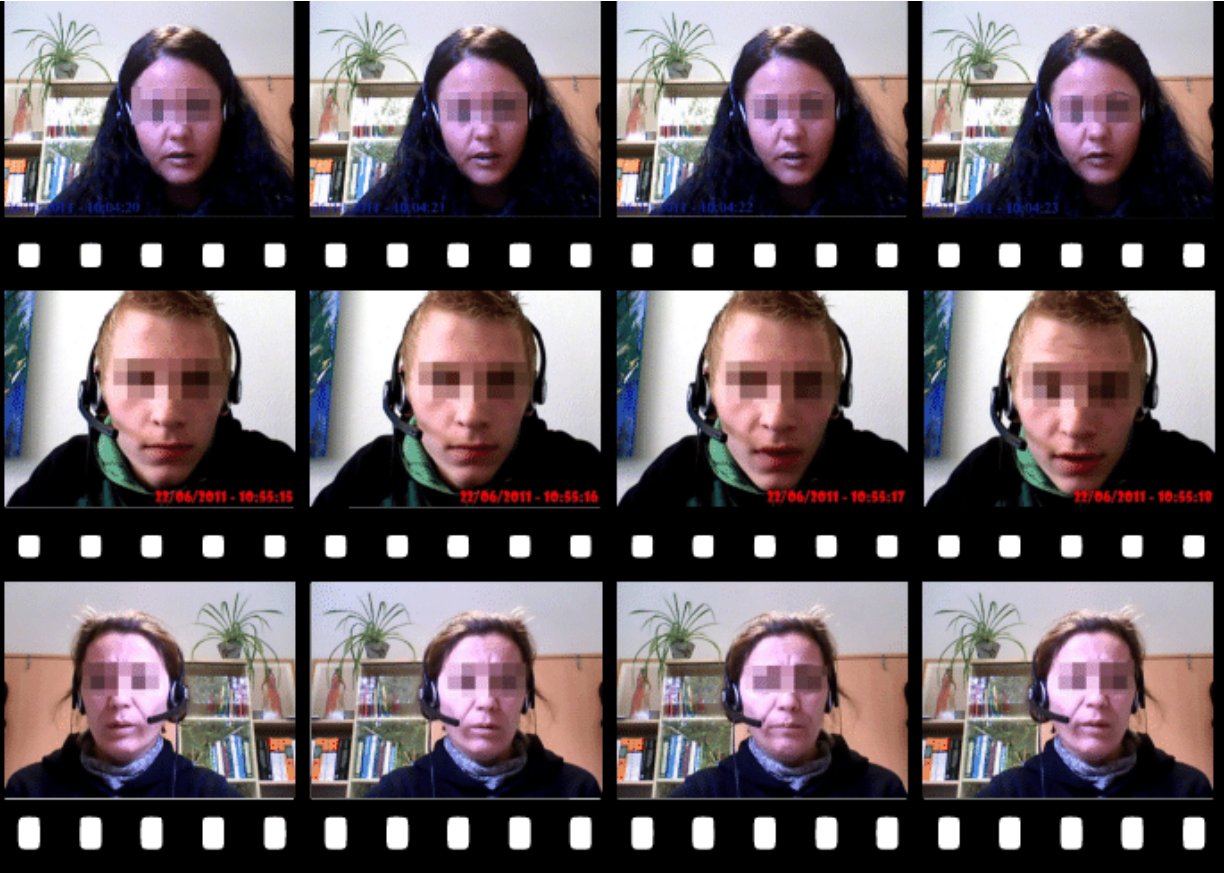
\includegraphics[width=0.8\linewidth]{figures/depression/facial-AVEC.png}		
	\caption{
	Samples from AVEC datasets.
	}
	\label{facial-AVEC}
\end{figure}

\begin{figure}[tbp]
	\centering	
	\label{fig_hard_case1}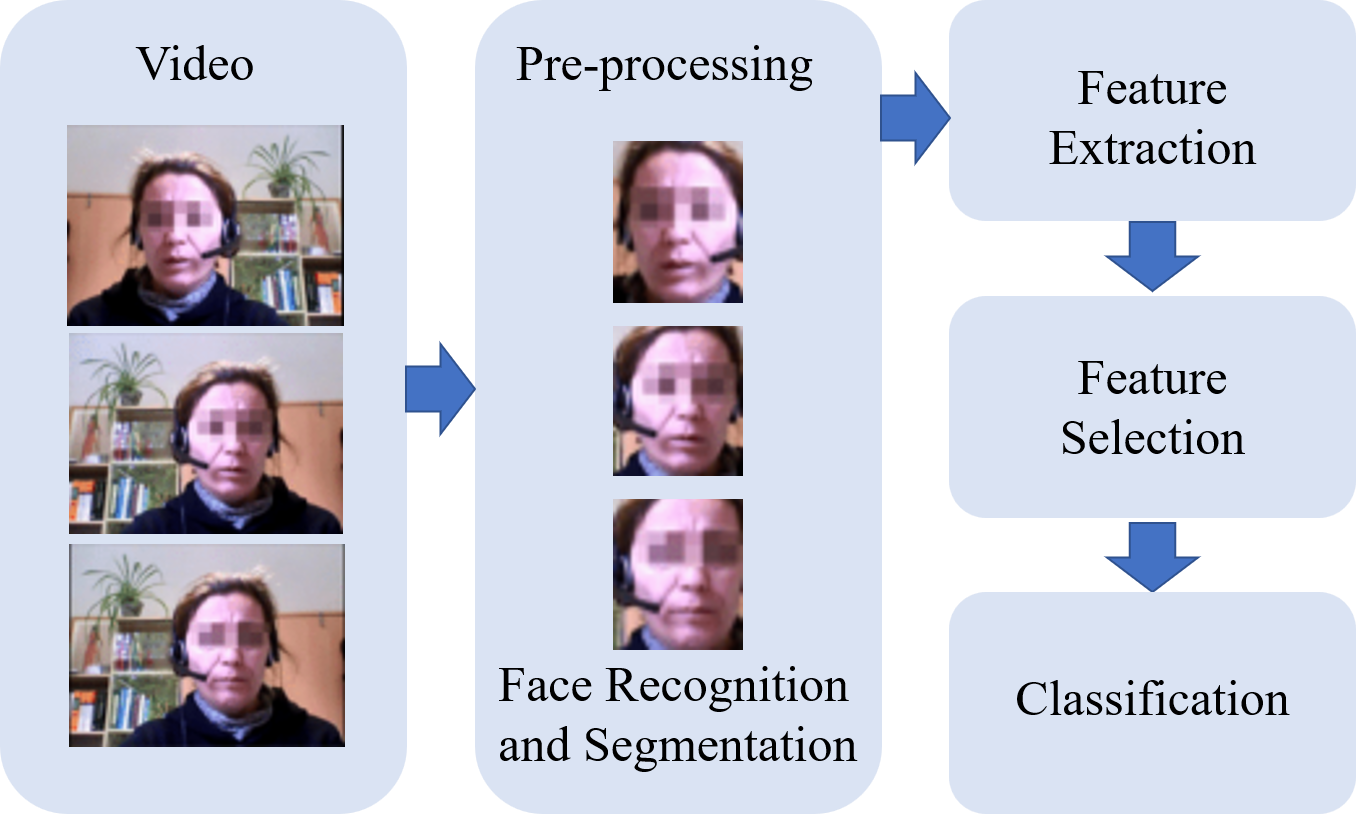
\includegraphics[width=0.8\linewidth]{figures/depression/facial.png}		
	\caption{
	Flow chart of expression-based depression recognition model.
	}
	\label{facial}
\end{figure}

A person's personality and mood can be seen from his face, and some studies have found that the appearance and temperament of patients with depression are also different from ordinary people.
Zhu et al.~\cite{0Identifying} research team of the institute of psychology of the Chinese Academy of Sciences studied 100 people with mental diseases. They asked 100 patients to read neutral articles through a special technology. From the research process, it was found that these patients frowned and drooped corners of their mouths when reading aloud, and a few tears appeared in their eyes, just like crying, looking very sad.

In order to study the relationship between patients' depression severity and facial expression over time, Girard et al.~\cite{2013Social} designed a study to track the subjects for two years, and collected the data of 36 patients with severe depression at the beginning and reduced symptoms after two years. Through the analysis of facial expressions in video data by manual and automatic systems, it showed that the automatic coding of Facial Action Coding System (FACS) action units is highly consistent with the manual coding, and showed a similar effect in the change of depression severity over time.

The results showed that when the severity of patients' symptoms was high, participants made more facial expressions related to contempt and smiled less, and those smiles were more likely to be accompanied by facial actions related to contempt. These results were consistent with the performance of Exchange-Oriented Withdrawal in the "Social Risk Hypothesis" of depression, indicating that patients with depression show more withdrawal in social intercourse. According to this hypothesis, when patients have severe symptoms, they will stay away from others to protect themselves from expected rejection, contempt and social exclusion~\cite{2005Emotion,BYLSMA2008676,2017Facial}.

\subsubsection{Facial expression depression recognition based on machine learning}
\label{sec_fquality}
%%%%%%%%%%%%%%%%%%%%%%%%%%%%%%%%%%%%%%%

To achieve depression recognition from facial images, traditional solutions for vision-based automatic depression diagnosis systems usually include several steps as shown in Fig \ref{facial}: first, facial images are recognized and segmented from the raw video data, then features are extracted, and finally the features are fed into a classifier for classification or regression.


Machine learning can be divided into traditional machine based on the depth of the model structure learning and deep learning, which are now often applied to tasks such as vision and speech on tasks such as vision and speech. While traditional machine learning algorithms are suitable for small amounts of data, deep learning has higher performance on larger data sets.
%Machine learning is used in facial feature feature extraction and classification in facial features research.

Traditional machine learning methods such as SVM, naive Bayes (NB), RF and logistic regression (LR) are the most commonly used classifiers in the study of facial features of depressed patients~\cite{2017A,2018A,2020Automatic,2021Classifying}.


\subsubsection{Facial expression depression recognition based on deep learning}
\label{sec_fquality}
%%%%%%%%%%%%%%%%%%%%%%%%%%%%%%%%%%%%%%%

Convolutional neural networks (CNNs) are the most commonly used deep learning networks for facial recognition research in recent years. Many researches based on CNN and its innovative architectures such as three-dimensional CNN (C3D), modality separation networks (MSN), deep residual regression convolutional neural networks (DRR-CNN) for recognizing, classifying, and predicting human emotions, as well as exploring how facial action intensity changes from low to high levels of emotion~\cite{2019Combining,2019Multi,2020Encoding,2020A,2020Visually,2020Depression}. There are also studies that build on CNNs by embedding expectation loss into ResNet-50, a residual neural network, for distributional learning, which allows exploring the sequential relationship between facial images and depression levels to better predict depression levels~\cite{2019Depression2}.

Recurrent neural networks (RNN)~\cite{8466881} are suitable for learning for time series, better simulate feature changes to improve classification accuracy, and when combined with CNNs can also handle computer vision problems that contain sequential inputs. The LSTM~\cite{2017Exploring}~\cite{2020Automatic2} is also commonly used in facial recognition research, and is suitable for processing and predicting important events with very long intervals and delays in time series, which is more in line with the detection of continuously changing emotions and close to the clinical reality.

Depression alters many behaviors, among which the face presents most of people's nonverbal information. Therefore, facial expressions are highly informative characteristic indicators in the diagnosis of depression, providing more support for clinical studies of depression and offering the possibility of automated detection of depression.


\subsubsection{Performance Comparison}
%\label{sec\_fquality}
%%%%%%%%%%%%%%%%%%%%%%%%%%%%%%%%%%%%%%%
Table \ref{tab4} summarizes the results of the experiments on the detection of depression based on facial expressions, including the source and name of the method, the data set used (- means the data used were collected by ourselves), the evaluation criteria of the experimental results, including the classification criteria Accuracy, F1 Score Precision, Recall, the evaluation criteria of depression severity by depression scale mean absolute error (MAE) and root mean square error (RMSE), and Average Error for regression scale scores.

The AVEC competition has greatly advanced research on depression detection based on behavioral performance, and more and more deep algorithms have been applied to depression recognition tasks, all with good results.

%%%%%%%%%%%%%%%%%%%%%%%%%%%%%%%%%%%%%%

\begin{table*}
\centering
\caption{Experimental results based on facial}
\label{tab4}
\begin{tabular}{l|l|l|llll|ll|ll}

\hline
\multicolumn{1}{c|}{\multirow{2}{*}{ID}} & \multicolumn{1}{c|}{\multirow{2}{*}{Method}}                         & \multirow{2}{*}{Dataset} & \multicolumn{4}{c|}{Classification}       & \multicolumn{2}{c|}{\shortstack{depression severity \\estimation}} & \multicolumn{2}{c}{Regression}                                \\
                  &                                                                        &                          & Accuracy & F1 Score & Precision & Recall & \multicolumn{1}{c}{RMSE} & \multicolumn{1}{c|}{MAE} & \multicolumn{1}{c}{Scale} & \multicolumn{1}{c}{Average Error} \\
\hline
1                                       & AVEC2013 baseline~\cite{10.1145/2512530.2512533}                                                               & AVEC2013                                     & -        & -          & -         & -      & 13.61                    & 10.88                   & -         & -                  \\
2                                       & AVEC2014 baseline~\cite{10.1145/2661806.2661807}                                                               & AVEC2014                                     & -        & -          & -         & -      & 10.86                    & 8.86                    & -         & -                  \\
3                                       & LPQ+Geo~\cite{2014Eyes}                                                                                        & AVEC2013                                     & -        & -          & -         & -      & 9.72                     & 7.86                    & -         & -                  \\
4                                       & MHH+PLS~\cite{ 2014Automatic}                                                                                  & AVEC2014                                     & -        & -          & -         & -      & 10.5                     & 8.44                    & -         & -                  \\
5                                       & LPQ-TOP+MFA~\cite{2015Automated}                                                                               & AVEC2013                                     & -        & -          & -         & -      & 10.27                    & 8.22                    & -         & -                  \\
6                                       & AVEC2016 baseline~\cite{valstar2016avec}                                                                                     & DAIC-WOZ                                     & -        & 50.00      & 60.00     & 42.80  & 7.13                     & 5.88                    & PHQ       & 7.13               \\
7                                       & Williamson et al.~\cite{2016Detecting}                                                                         & DAIC-WOZ                                     & -        & 53.00      & -         & -      & -                        & -                       & PHQ       & 5.33               \\
8                                       & AVEC2017 baseline~\cite{ringeval2017avec}                                                                      & AVEC2017                                     & -        & -          & -         & -      & 6.97                     & 6.12                    & -         & -                  \\
9                                      & LSTM~\cite{ 2017Exploring}                                                                                     & -                                            & 67.7     & -          & -         & -      & -                        & -                       & -         & -                  \\
10                                      & Two DCNN~\cite{2017Automated}                                                                                  & AVEC2013                                     & -        & -          & -         & -      & 9.82                     & 7.58                    & -         & -                  \\
11                                      & Two DCNN~\cite{2017Automated}                                                                                  & AVEC2014                                     & -        & -          & -         & -      & 9.55                     & 7.47                    & -         & -                  \\
12                                      & SVM+NB+RF~\cite{2018A}                                                                                         & -                                            & 69.10    & -          & -         & -      & -                        & -                       & -         & -                  \\
13                                      & AVEC2019 baseline~\cite{ ringeval2019avec}                                                                     & AVEC201                                      & -        & -          & -         & -      & 8.01                     & -                       & -         & -                  \\
14                                      & C3D~\cite{2019Combining}                                                                                       & AVEC2013                                     & -        & -          & -         & -      & 8.26                     & 6.40                    & -         & -                  \\
15                                      & C3D~\cite{2019Combining}                                                                                       & AVEC2014                                     & -        & -          & -         & -      & 8.31                     & 6.59                    & -         & -                  \\
16                                      & Ray et al.~\cite{ray2019multi}                                                                                 & -                                            & -        & -          & -         & -      & 8.95                     & -                       & -         & -                  \\
17                                      & ResNet-50~\cite{2019Depression2}                                                                               & AVEC2013                                     & -        & -          & -         & -      & 8.25                     & 6.30                    & -         & -                  \\
18                                      & ResNet-50~\cite{2019Depression2}                                                                               & AVEC2014                                     & -        & -          & -         & -      & 8.23                     & 6.15                    & -         & -                  \\
19                                      & ResNet-50+pool~\cite{2019Learning}                                                                             & AVEC2014                                     & -        & -          & -         & -      & 8.43                     & 6.37                    & -         & -                  \\
20                                      & MSN~\cite{ 2020A}                                                                                              & AVEC2013                                     & -        & -          & -         & -      & 7.90                     & 5.98                    & -         & -                  \\
21                                      & MSN~\cite{ 2020A}                                                                                              & AVEC2014                                     & -        & -          & -         & -      & 7.61                     & 5.82                    & -         & -                  \\
22                                      & MR-DepressNet~\cite{2020Visually}                                                                              & AVEC2013                                     & -        & -          & -         & -      & 8.28                     & 6.20                    & -         & -                  \\
23                                      & MR-DepressNet~\cite{2020Visually}                                                                              & AVEC2014                                     & -        & -          & -         & -      & 8.39                     & 6.21                    & -         & -                  \\
24                                      & Two-Stream model~\cite{2020Encoding}                                                                           & AVEC2013                                     & -        & -          & -         & -      & 7.97                     & 5.96                    & -         & -                  \\
25                                      & Two-Stream model~\cite{2020Encoding}                                                                           & AVEC2014                                     & -        & -          & -         & -      & 7.94                     & 6.20                    & -         & -                  \\
26                                      & CNN~\cite{2020Automatic}                                                                                       & -                                            & 66.45    & -          & -         & -      & -                        & -                       & -         & -                  \\
27                                      & SS-LSTM-MIL~\cite{2020Automatic2}                                                                              & DAC-WOZ                                      & -        & 78.3       & 81.80     & 75.00  & -                        & -                       & -         & -                  \\
28                                      & \begin{tabular}[c]{@{}l@{}}RNN-C3D Tight-Face \& Loose-Face\\ \\weighted merge~\cite{8466881}\end{tabular} & AVEC2013                                     & -        & -          & -         & -      & 9.28                     & 7.37                    & -         & -                  \\
29                                      & \begin{tabular}[c]{@{}l@{}}RNN-C3D Tight-Face \& Loose-Face\\ \\weighted merge~\cite{8466881}\end{tabular} & AVEC2014                                     & -        & -          & -         & -      & 9.20                     & 7.22                    & -         & -                 \\
\hline

\end{tabular}
\end{table*}



\ifx\allfiles\undefined
\input{tnnls\_suffix}
\fi
